\documentclass[1p]{elsarticle_modified}
%\bibliographystyle{elsarticle-num}

%\usepackage[colorlinks]{hyperref}
%\usepackage{abbrmath_seonhwa} %\Abb, \Ascr, \Acal ,\Abf, \Afrak
\usepackage{amsfonts}
\usepackage{amssymb}
\usepackage{amsmath}
\usepackage{amsthm}
\usepackage{scalefnt}
\usepackage{amsbsy}
\usepackage{kotex}
\usepackage{caption}
\usepackage{subfig}
\usepackage{color}
\usepackage{graphicx}
\usepackage{xcolor} %% white, black, red, green, blue, cyan, magenta, yellow
\usepackage{float}
\usepackage{setspace}
\usepackage{hyperref}

\usepackage{tikz}
\usetikzlibrary{arrows}

\usepackage{multirow}
\usepackage{array} % fixed length table
\usepackage{hhline}

%%%%%%%%%%%%%%%%%%%%%
\makeatletter
\renewcommand*\env@matrix[1][\arraystretch]{%
	\edef\arraystretch{#1}%
	\hskip -\arraycolsep
	\let\@ifnextchar\new@ifnextchar
	\array{*\c@MaxMatrixCols c}}
\makeatother %https://tex.stackexchange.com/questions/14071/how-can-i-increase-the-line-spacing-in-a-matrix
%%%%%%%%%%%%%%%

\usepackage[normalem]{ulem}

\newcommand{\msout}[1]{\ifmmode\text{\sout{\ensuremath{#1}}}\else\sout{#1}\fi}
%SOURCE: \msout is \stkout macro in https://tex.stackexchange.com/questions/20609/strikeout-in-math-mode

\newcommand{\cancel}[1]{
	\ifmmode
	{\color{red}\msout{#1}}
	\else
	{\color{red}\sout{#1}}
	\fi
}

\newcommand{\add}[1]{
	{\color{blue}\uwave{#1}}
}

\newcommand{\replace}[2]{
	\ifmmode
	{\color{red}\msout{#1}}{\color{blue}\uwave{#2}}
	\else
	{\color{red}\sout{#1}}{\color{blue}\uwave{#2}}
	\fi
}

\newcommand{\Sol}{\mathcal{S}} %segment
\newcommand{\D}{D} %diagram
\newcommand{\A}{\mathcal{A}} %arc


%%%%%%%%%%%%%%%%%%%%%%%%%%%%%5 test

\def\sl{\operatorname{\textup{SL}}(2,\Cbb)}
\def\psl{\operatorname{\textup{PSL}}(2,\Cbb)}
\def\quan{\mkern 1mu \triangleright \mkern 1mu}

\theoremstyle{definition}
\newtheorem{thm}{Theorem}[section]
\newtheorem{prop}[thm]{Proposition}
\newtheorem{lem}[thm]{Lemma}
\newtheorem{ques}[thm]{Question}
\newtheorem{cor}[thm]{Corollary}
\newtheorem{defn}[thm]{Definition}
\newtheorem{exam}[thm]{Example}
\newtheorem{rmk}[thm]{Remark}
\newtheorem{alg}[thm]{Algorithm}

\newcommand{\I}{\sqrt{-1}}
\begin{document}

%\begin{frontmatter}
%
%\title{Boundary parabolic representations of knots up to 8 crossings}
%
%%% Group authors per affiliation:
%\author{Yunhi Cho} 
%\address{Department of Mathematics, University of Seoul, Seoul, Korea}
%\ead{yhcho@uos.ac.kr}
%
%
%\author{Seonhwa Kim} %\fnref{s_kim}}
%\address{Center for Geometry and Physics, Institute for Basic Science, Pohang, 37673, Korea}
%\ead{ryeona17@ibs.re.kr}
%
%\author{Hyuk Kim}
%\address{Department of Mathematical Sciences, Seoul National University, Seoul 08826, Korea}
%\ead{hyukkim@snu.ac.kr}
%
%\author{Seokbeom Yoon}
%\address{Department of Mathematical Sciences, Seoul National University, Seoul, 08826,  Korea}
%\ead{sbyoon15@snu.ac.kr}
%
%\begin{abstract}
%We find all boundary parabolic representation of knots up to 8 crossings.
%
%\end{abstract}
%\begin{keyword}
%    \MSC[2010] 57M25 
%\end{keyword}
%
%\end{frontmatter}

%\linenumbers
%\tableofcontents
%
\newcommand\colored[1]{\textcolor{white}{\rule[-0.35ex]{0.8em}{1.4ex}}\kern-0.8em\color{red} #1}%
%\newcommand\colored[1]{\textcolor{white}{ #1}\kern-2.17ex	\textcolor{white}{ #1}\kern-1.81ex	\textcolor{white}{ #1}\kern-2.15ex\color{red}#1	}

{\Large $\underline{12n_{0085}~(K12n_{0085})}$}

\setlength{\tabcolsep}{10pt}
\renewcommand{\arraystretch}{1.6}
\vspace{1cm}\begin{tabular}{m{100pt}>{\centering\arraybackslash}m{274pt}}
\multirow{5}{120pt}{
	\centering
	\includegraphics[width=112pt]{../../../GIT/diagram.site/Diagrams/png/2174_12n_0085.png}\\
\ \ \ A knot diagram\footnotemark}&
\allowdisplaybreaks
\textbf{Linearized knot diagam} \\
\cline{2-2}
 &
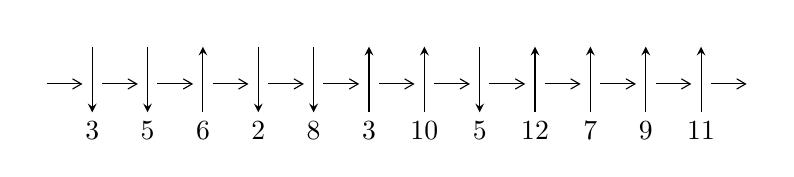
\begin{tikzpicture}[x=20pt, y=17pt]
	% nodes
	\node (C0) at (0, 0) {};
	\node (C1) at (1, 0) {};
	\node (C1U) at (1, +1) {};
	\node (C1D) at (1, -1) {3};

	\node (C2) at (2, 0) {};
	\node (C2U) at (2, +1) {};
	\node (C2D) at (2, -1) {5};

	\node (C3) at (3, 0) {};
	\node (C3U) at (3, +1) {};
	\node (C3D) at (3, -1) {6};

	\node (C4) at (4, 0) {};
	\node (C4U) at (4, +1) {};
	\node (C4D) at (4, -1) {2};

	\node (C5) at (5, 0) {};
	\node (C5U) at (5, +1) {};
	\node (C5D) at (5, -1) {8};

	\node (C6) at (6, 0) {};
	\node (C6U) at (6, +1) {};
	\node (C6D) at (6, -1) {3};

	\node (C7) at (7, 0) {};
	\node (C7U) at (7, +1) {};
	\node (C7D) at (7, -1) {10};

	\node (C8) at (8, 0) {};
	\node (C8U) at (8, +1) {};
	\node (C8D) at (8, -1) {5};

	\node (C9) at (9, 0) {};
	\node (C9U) at (9, +1) {};
	\node (C9D) at (9, -1) {12};

	\node (C10) at (10, 0) {};
	\node (C10U) at (10, +1) {};
	\node (C10D) at (10, -1) {7};

	\node (C11) at (11, 0) {};
	\node (C11U) at (11, +1) {};
	\node (C11D) at (11, -1) {9};

	\node (C12) at (12, 0) {};
	\node (C12U) at (12, +1) {};
	\node (C12D) at (12, -1) {11};
	\node (C13) at (13, 0) {};

	% arrows
	\draw[->,>={angle 60}]
	(C0) edge (C1) (C1) edge (C2) (C2) edge (C3) (C3) edge (C4) (C4) edge (C5) (C5) edge (C6) (C6) edge (C7) (C7) edge (C8) (C8) edge (C9) (C9) edge (C10) (C10) edge (C11) (C11) edge (C12) (C12) edge (C13) ;	\draw[->,>=stealth]
	(C1U) edge (C1D) (C2U) edge (C2D) (C3D) edge (C3U) (C4U) edge (C4D) (C5U) edge (C5D) (C6D) edge (C6U) (C7D) edge (C7U) (C8U) edge (C8D) (C9D) edge (C9U) (C10D) edge (C10U) (C11D) edge (C11U) (C12D) edge (C12U) ;
	\end{tikzpicture} \\
\hhline{~~} \\& 
\textbf{Solving Sequence} \\ \cline{2-2} 
 &
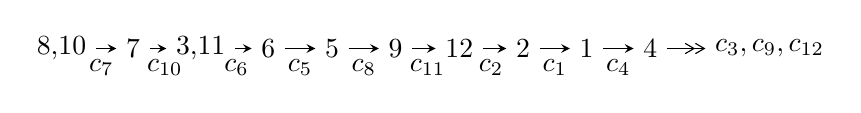
\begin{tikzpicture}[x=23pt, y=7pt]
	% node
	\node (A0) at (-1/8, 0) {8,10};
	\node (A1) at (1, 0) {7};
	\node (A2) at (33/16, 0) {3,11};
	\node (A3) at (25/8, 0) {6};
	\node (A4) at (33/8, 0) {5};
	\node (A5) at (41/8, 0) {9};
	\node (A6) at (49/8, 0) {12};
	\node (A7) at (57/8, 0) {2};
	\node (A8) at (65/8, 0) {1};
	\node (A9) at (73/8, 0) {4};
	\node (C1) at (1/2, -1) {$c_{7}$};
	\node (C2) at (3/2, -1) {$c_{10}$};
	\node (C3) at (21/8, -1) {$c_{6}$};
	\node (C4) at (29/8, -1) {$c_{5}$};
	\node (C5) at (37/8, -1) {$c_{8}$};
	\node (C6) at (45/8, -1) {$c_{11}$};
	\node (C7) at (53/8, -1) {$c_{2}$};
	\node (C8) at (61/8, -1) {$c_{1}$};
	\node (C9) at (69/8, -1) {$c_{4}$};
	\node (A10) at (11, 0) {$c_{3},c_{9},c_{12}$};

	% edge
	\draw[->,>=stealth]	
	(A0) edge (A1) (A1) edge (A2) (A2) edge (A3) (A3) edge (A4) (A4) edge (A5) (A5) edge (A6) (A6) edge (A7) (A7) edge (A8) (A8) edge (A9) ;
	\draw[->>,>={angle 60}]	
	(A9) edge (A10);
\end{tikzpicture} \\ 

\end{tabular} \\

\footnotetext{
The image of knot diagram is generated by the software ``\textbf{Draw programme}" developed by Andrew Bartholomew(\url{http://www.layer8.co.uk/maths/draw/index.htm\#Running-draw}), where we modified some parts for our purpose(\url{https://github.com/CATsTAILs/LinksPainter}).
}\phantom \\ \newline 
\centering \textbf{Ideals for irreducible components\footnotemark of $X_{\text{par}}$} 
 
\begin{align*}
I^u_{1}&=\langle 
-8.01204\times10^{90} u^{45}+1.50405\times10^{91} u^{44}+\cdots+3.33019\times10^{91} b-2.86123\times10^{92},\\
\phantom{I^u_{1}}&\phantom{= \langle  }-5.16653\times10^{90} u^{45}+9.63398\times10^{90} u^{44}+\cdots+3.33019\times10^{91} a-3.97217\times10^{92},\\
\phantom{I^u_{1}}&\phantom{= \langle  }u^{46}-2 u^{45}+\cdots+32 u+32\rangle \\
I^u_{2}&=\langle 
u^8-2 u^7+3 u^6-3 u^5+4 u^4-4 u^3+3 u^2+b-2 u+1,\\
\phantom{I^u_{2}}&\phantom{= \langle  }3 u^8-4 u^7+8 u^6-7 u^5+13 u^4-9 u^3+11 u^2+a-6 u+6,\;u^9- u^8+2 u^7- u^6+3 u^5- u^4+2 u^3+u+1\rangle \\
\\
I^v_{1}&=\langle 
a,\;-16 v^4+47 v^3-36 v^2+29 b+104 v+5,\;v^5-3 v^4+3 v^3-8 v^2+v-1\rangle \\
\end{align*}
\raggedright * 3 irreducible components of $\dim_{\mathbb{C}}=0$, with total 60 representations.\\
\footnotetext{All coefficients of polynomials are rational numbers. But the coefficients are sometimes approximated in decimal forms when there is not enough margin.}
\newpage
\renewcommand{\arraystretch}{1}
\centering \section*{I. $I^u_{1}= \langle -8.01\times10^{90} u^{45}+1.50\times10^{91} u^{44}+\cdots+3.33\times10^{91} b-2.86\times10^{92},\;-5.17\times10^{90} u^{45}+9.63\times10^{90} u^{44}+\cdots+3.33\times10^{91} a-3.97\times10^{92},\;u^{46}-2 u^{45}+\cdots+32 u+32 \rangle$}
\flushleft \textbf{(i) Arc colorings}\\
\begin{tabular}{m{7pt} m{180pt} m{7pt} m{180pt} }
\flushright $a_{8}=$&$\begin{pmatrix}1\\0\end{pmatrix}$ \\
\flushright $a_{10}=$&$\begin{pmatrix}0\\u\end{pmatrix}$ \\
\flushright $a_{7}=$&$\begin{pmatrix}1\\u^2\end{pmatrix}$ \\
\flushright $a_{3}=$&$\begin{pmatrix}0.155142 u^{45}-0.289292 u^{44}+\cdots+3.45866 u+11.9278\\0.240588 u^{45}-0.451642 u^{44}+\cdots+31.6377 u+8.59181\end{pmatrix}$ \\
\flushright $a_{11}=$&$\begin{pmatrix}u\\u^3+u\end{pmatrix}$ \\
\flushright $a_{6}=$&$\begin{pmatrix}0.180370 u^{45}-0.347609 u^{44}+\cdots+22.1880 u+3.90329\\0.00906533 u^{45}-0.0528530 u^{44}+\cdots-1.97758 u-5.86471\end{pmatrix}$ \\
\flushright $a_{5}=$&$\begin{pmatrix}0.189435 u^{45}-0.400462 u^{44}+\cdots+20.2104 u-1.96143\\0.00906533 u^{45}-0.0528530 u^{44}+\cdots-1.97758 u-5.86471\end{pmatrix}$ \\
\flushright $a_{9}=$&$\begin{pmatrix}0.0972359 u^{45}-0.101045 u^{44}+\cdots+18.1876 u+12.7399\\0.0831514 u^{45}-0.0596108 u^{44}+\cdots+23.5834 u+14.7786\end{pmatrix}$ \\
\flushright $a_{12}=$&$\begin{pmatrix}0.0216467 u^{45}-0.00784512 u^{44}+\cdots+11.4970 u+5.02842\\0.118455 u^{45}-0.115438 u^{44}+\cdots+27.8576 u+16.6339\end{pmatrix}$ \\
\flushright $a_{2}=$&$\begin{pmatrix}-0.0465827 u^{45}+0.0735841 u^{44}+\cdots-26.1646 u+6.17270\\0.203398 u^{45}-0.521213 u^{44}+\cdots+12.7874 u-10.4351\end{pmatrix}$ \\
\flushright $a_{1}=$&$\begin{pmatrix}0.0140845 u^{45}-0.0414345 u^{44}+\cdots-5.39582 u-2.03877\\-0.0959655 u^{45}+0.0891363 u^{44}+\cdots-23.6096 u-14.3541\end{pmatrix}$ \\
\flushright $a_{4}=$&$\begin{pmatrix}0.422424 u^{45}-0.812824 u^{44}+\cdots+41.9060 u+18.8214\\-0.0860042 u^{45}+0.279668 u^{44}+\cdots-6.21471 u+14.2803\end{pmatrix}$\\&\end{tabular}
\flushleft \textbf{(ii) Obstruction class $= -1$}\\~\\
\flushleft \textbf{(iii) Cusp Shapes $= 2.27338 u^{45}-5.41938 u^{44}+\cdots+115.558 u-6.90034$}\\~\\
\newpage\renewcommand{\arraystretch}{1}
\flushleft \textbf{(iv) u-Polynomials at the component}\newline \\
\begin{tabular}{m{50pt}|m{274pt}}
Crossings & \hspace{64pt}u-Polynomials at each crossing \\
\hline $$\begin{aligned}c_{1}\end{aligned}$$&$\begin{aligned}
&u^{46}+61 u^{45}+\cdots+62504 u+1
\end{aligned}$\\
\hline $$\begin{aligned}c_{2},c_{4}\end{aligned}$$&$\begin{aligned}
&u^{46}-11 u^{45}+\cdots+260 u-1
\end{aligned}$\\
\hline $$\begin{aligned}c_{3},c_{6}\end{aligned}$$&$\begin{aligned}
&u^{46}+8 u^{45}+\cdots+9216 u+512
\end{aligned}$\\
\hline $$\begin{aligned}c_{5},c_{8}\end{aligned}$$&$\begin{aligned}
&u^{46}-3 u^{45}+\cdots+2 u-1
\end{aligned}$\\
\hline $$\begin{aligned}c_{7},c_{10}\end{aligned}$$&$\begin{aligned}
&u^{46}+2 u^{45}+\cdots-32 u+32
\end{aligned}$\\
\hline $$\begin{aligned}c_{9},c_{11}\end{aligned}$$&$\begin{aligned}
&u^{46}+7 u^{45}+\cdots+4 u+1
\end{aligned}$\\
\hline $$\begin{aligned}c_{12}\end{aligned}$$&$\begin{aligned}
&u^{46}-17 u^{45}+\cdots-22 u+1
\end{aligned}$\\
\hline
\end{tabular}\\~\\
\newpage\renewcommand{\arraystretch}{1}
\flushleft \textbf{(v) Riley Polynomials at the component}\newline \\
\begin{tabular}{m{50pt}|m{274pt}}
Crossings & \hspace{64pt}Riley Polynomials at each crossing \\
\hline $$\begin{aligned}c_{1}\end{aligned}$$&$\begin{aligned}
&y^{46}-141 y^{45}+\cdots-3903085204 y+1
\end{aligned}$\\
\hline $$\begin{aligned}c_{2},c_{4}\end{aligned}$$&$\begin{aligned}
&y^{46}-61 y^{45}+\cdots-62504 y+1
\end{aligned}$\\
\hline $$\begin{aligned}c_{3},c_{6}\end{aligned}$$&$\begin{aligned}
&y^{46}+60 y^{45}+\cdots-71827456 y+262144
\end{aligned}$\\
\hline $$\begin{aligned}c_{5},c_{8}\end{aligned}$$&$\begin{aligned}
&y^{46}- y^{45}+\cdots-32 y+1
\end{aligned}$\\
\hline $$\begin{aligned}c_{7},c_{10}\end{aligned}$$&$\begin{aligned}
&y^{46}+36 y^{45}+\cdots+8704 y+1024
\end{aligned}$\\
\hline $$\begin{aligned}c_{9},c_{11}\end{aligned}$$&$\begin{aligned}
&y^{46}-17 y^{45}+\cdots-22 y+1
\end{aligned}$\\
\hline $$\begin{aligned}c_{12}\end{aligned}$$&$\begin{aligned}
&y^{46}+31 y^{45}+\cdots+246 y+1
\end{aligned}$\\
\hline
\end{tabular}\\~\\
\newpage\flushleft \textbf{(vi) Complex Volumes and Cusp Shapes}
$$\begin{array}{c|c|c}  
\text{Solutions to }I^u_{1}& \I (\text{vol} + \sqrt{-1}CS) & \text{Cusp shape}\\
 \hline 
\begin{aligned}
u &= -0.378169 + 0.944081 I \\
a &= \phantom{-}0.311249 - 0.267542 I \\
b &= \phantom{-}0.391023 - 0.209753 I\end{aligned}
 & \phantom{-}0.00959 - 1.79095 I & \phantom{-}3.07595 + 1.44696 I \\ \hline\begin{aligned}
u &= -0.378169 - 0.944081 I \\
a &= \phantom{-}0.311249 + 0.267542 I \\
b &= \phantom{-}0.391023 + 0.209753 I\end{aligned}
 & \phantom{-}0.00959 + 1.79095 I & \phantom{-}3.07595 - 1.44696 I \\ \hline\begin{aligned}
u &= \phantom{-}0.733270 + 0.623347 I \\
a &= \phantom{-}0.092842 + 0.753829 I \\
b &= -0.073700 + 0.162456 I\end{aligned}
 & \phantom{-}3.69426 - 1.19679 I & \phantom{-}10.96091 + 0.32680 I \\ \hline\begin{aligned}
u &= \phantom{-}0.733270 - 0.623347 I \\
a &= \phantom{-}0.092842 - 0.753829 I \\
b &= -0.073700 - 0.162456 I\end{aligned}
 & \phantom{-}3.69426 + 1.19679 I & \phantom{-}10.96091 - 0.32680 I \\ \hline\begin{aligned}
u &= -0.172617 + 1.096660 I \\
a &= \phantom{-}0.353108 - 0.099187 I \\
b &= -0.924288 - 0.155002 I\end{aligned}
 & -2.08149 - 2.37209 I & \phantom{-}2.00000 + 4.29323 I \\ \hline\begin{aligned}
u &= -0.172617 - 1.096660 I \\
a &= \phantom{-}0.353108 + 0.099187 I \\
b &= -0.924288 + 0.155002 I\end{aligned}
 & -2.08149 + 2.37209 I & \phantom{-}2.00000 - 4.29323 I \\ \hline\begin{aligned}
u &= \phantom{-}0.863631 + 0.008081 I \\
a &= \phantom{-}0.668878 - 0.492509 I \\
b &= \phantom{-}0.385328 + 1.024490 I\end{aligned}
 & -1.00247 + 2.85719 I & -1.18117 - 7.51903 I \\ \hline\begin{aligned}
u &= \phantom{-}0.863631 - 0.008081 I \\
a &= \phantom{-}0.668878 + 0.492509 I \\
b &= \phantom{-}0.385328 - 1.024490 I\end{aligned}
 & -1.00247 - 2.85719 I & -1.18117 + 7.51903 I \\ \hline\begin{aligned}
u &= \phantom{-}0.681454 + 1.055760 I \\
a &= \phantom{-}0.120812 + 0.262349 I \\
b &= \phantom{-}0.266053 - 0.121547 I\end{aligned}
 & \phantom{-}2.40464 + 6.60583 I & \phantom{-0.000000 } 0 \\ \hline\begin{aligned}
u &= \phantom{-}0.681454 - 1.055760 I \\
a &= \phantom{-}0.120812 - 0.262349 I \\
b &= \phantom{-}0.266053 + 0.121547 I\end{aligned}
 & \phantom{-}2.40464 - 6.60583 I & \phantom{-0.000000 } 0\\
 \hline 
 \end{array}$$\newpage$$\begin{array}{c|c|c}  
\text{Solutions to }I^u_{1}& \I (\text{vol} + \sqrt{-1}CS) & \text{Cusp shape}\\
 \hline 
\begin{aligned}
u &= -0.668016 + 0.132668 I \\
a &= \phantom{-}2.07679 - 1.43704 I \\
b &= \phantom{-}0.55122 - 1.51352 I\end{aligned}
 & -0.282269 + 0.067141 I & -3.72609 - 3.28540 I \\ \hline\begin{aligned}
u &= -0.668016 - 0.132668 I \\
a &= \phantom{-}2.07679 + 1.43704 I \\
b &= \phantom{-}0.55122 + 1.51352 I\end{aligned}
 & -0.282269 - 0.067141 I & -3.72609 + 3.28540 I \\ \hline\begin{aligned}
u &= -0.023048 + 1.365510 I \\
a &= -0.38400 - 1.87511 I \\
b &= \phantom{-}0.22263 + 1.67589 I\end{aligned}
 & -8.03047 + 4.15846 I & \phantom{-0.000000 } 0 \\ \hline\begin{aligned}
u &= -0.023048 - 1.365510 I \\
a &= -0.38400 + 1.87511 I \\
b &= \phantom{-}0.22263 - 1.67589 I\end{aligned}
 & -8.03047 - 4.15846 I & \phantom{-0.000000 } 0 \\ \hline\begin{aligned}
u &= -0.114821 + 0.599864 I \\
a &= \phantom{-}2.68162 + 4.45685 I \\
b &= -0.366474 - 1.006750 I\end{aligned}
 & \phantom{-}0.67146 + 1.37994 I & -4.76488 - 1.12257 I \\ \hline\begin{aligned}
u &= -0.114821 - 0.599864 I \\
a &= \phantom{-}2.68162 - 4.45685 I \\
b &= -0.366474 + 1.006750 I\end{aligned}
 & \phantom{-}0.67146 - 1.37994 I & -4.76488 + 1.12257 I \\ \hline\begin{aligned}
u &= -0.112394 + 1.389540 I \\
a &= -0.32079 - 1.75033 I \\
b &= \phantom{-}0.52928 + 2.75631 I\end{aligned}
 & -5.00017 - 2.00257 I & \phantom{-0.000000 } 0 \\ \hline\begin{aligned}
u &= -0.112394 - 1.389540 I \\
a &= -0.32079 + 1.75033 I \\
b &= \phantom{-}0.52928 - 2.75631 I\end{aligned}
 & -5.00017 + 2.00257 I & \phantom{-0.000000 } 0 \\ \hline\begin{aligned}
u &= -0.33097 + 1.38999 I \\
a &= \phantom{-}0.40326 + 1.52193 I \\
b &= \phantom{-}0.86712 - 2.24790 I\end{aligned}
 & -4.56947 - 3.99633 I & \phantom{-0.000000 } 0 \\ \hline\begin{aligned}
u &= -0.33097 - 1.38999 I \\
a &= \phantom{-}0.40326 - 1.52193 I \\
b &= \phantom{-}0.86712 + 2.24790 I\end{aligned}
 & -4.56947 + 3.99633 I & \phantom{-0.000000 } 0\\
 \hline 
 \end{array}$$\newpage$$\begin{array}{c|c|c}  
\text{Solutions to }I^u_{1}& \I (\text{vol} + \sqrt{-1}CS) & \text{Cusp shape}\\
 \hline 
\begin{aligned}
u &= \phantom{-}1.43559 + 0.20920 I \\
a &= \phantom{-}0.0826736 - 0.0873667 I \\
b &= -0.35430 + 1.77050 I\end{aligned}
 & -9.88679 - 7.22887 I & \phantom{-0.000000 } 0 \\ \hline\begin{aligned}
u &= \phantom{-}1.43559 - 0.20920 I \\
a &= \phantom{-}0.0826736 + 0.0873667 I \\
b &= -0.35430 - 1.77050 I\end{aligned}
 & -9.88679 + 7.22887 I & \phantom{-0.000000 } 0 \\ \hline\begin{aligned}
u &= -1.44123 + 0.24926 I \\
a &= \phantom{-}0.0867294 - 0.0859579 I \\
b &= -0.05866 + 1.66324 I\end{aligned}
 & -9.81126 - 1.05399 I & \phantom{-0.000000 } 0 \\ \hline\begin{aligned}
u &= -1.44123 - 0.24926 I \\
a &= \phantom{-}0.0867294 + 0.0859579 I \\
b &= -0.05866 - 1.66324 I\end{aligned}
 & -9.81126 + 1.05399 I & \phantom{-0.000000 } 0 \\ \hline\begin{aligned}
u &= -0.059330 + 0.523960 I \\
a &= \phantom{-}0.581860 - 0.155990 I \\
b &= \phantom{-}0.354786 - 0.661801 I\end{aligned}
 & -0.00303 - 1.48232 I & -0.37531 + 3.95565 I \\ \hline\begin{aligned}
u &= -0.059330 - 0.523960 I \\
a &= \phantom{-}0.581860 + 0.155990 I \\
b &= \phantom{-}0.354786 + 0.661801 I\end{aligned}
 & -0.00303 + 1.48232 I & -0.37531 - 3.95565 I \\ \hline\begin{aligned}
u &= -0.518539\phantom{ +0.000000I} \\
a &= \phantom{-}1.22775\phantom{ +0.000000I} \\
b &= \phantom{-}0.266871\phantom{ +0.000000I}\end{aligned}
 & \phantom{-}1.19409\phantom{ +0.000000I} & \phantom{-}8.46120\phantom{ +0.000000I} \\ \hline\begin{aligned}
u &= \phantom{-}0.468629 + 0.218617 I \\
a &= \phantom{-}2.90732 - 0.59799 I \\
b &= -0.422461 + 0.238430 I\end{aligned}
 & -2.59187 - 0.05584 I & -4.82458 - 1.57408 I \\ \hline\begin{aligned}
u &= \phantom{-}0.468629 - 0.218617 I \\
a &= \phantom{-}2.90732 + 0.59799 I \\
b &= -0.422461 - 0.238430 I\end{aligned}
 & -2.59187 + 0.05584 I & -4.82458 + 1.57408 I \\ \hline\begin{aligned}
u &= -0.036031 + 0.497495 I \\
a &= \phantom{-}0.0857590 - 0.0907207 I \\
b &= -0.486106 + 1.121140 I\end{aligned}
 & -4.57386 - 4.46577 I & -14.2933 + 6.3376 I\\
 \hline 
 \end{array}$$\newpage$$\begin{array}{c|c|c}  
\text{Solutions to }I^u_{1}& \I (\text{vol} + \sqrt{-1}CS) & \text{Cusp shape}\\
 \hline 
\begin{aligned}
u &= -0.036031 - 0.497495 I \\
a &= \phantom{-}0.0857590 + 0.0907207 I \\
b &= -0.486106 - 1.121140 I\end{aligned}
 & -4.57386 + 4.46577 I & -14.2933 - 6.3376 I \\ \hline\begin{aligned}
u &= -0.01432 + 1.50322 I \\
a &= \phantom{-}0.01812 - 1.61025 I \\
b &= -0.329831 + 1.321610 I\end{aligned}
 & -6.74889 - 1.48702 I & \phantom{-0.000000 } 0 \\ \hline\begin{aligned}
u &= -0.01432 - 1.50322 I \\
a &= \phantom{-}0.01812 + 1.61025 I \\
b &= -0.329831 - 1.321610 I\end{aligned}
 & -6.74889 + 1.48702 I & \phantom{-0.000000 } 0 \\ \hline\begin{aligned}
u &= \phantom{-}0.42976 + 1.47936 I \\
a &= -0.49516 + 1.50593 I \\
b &= -0.55785 - 1.32892 I\end{aligned}
 & -5.92831 + 7.90364 I & \phantom{-0.000000 } 0 \\ \hline\begin{aligned}
u &= \phantom{-}0.42976 - 1.47936 I \\
a &= -0.49516 - 1.50593 I \\
b &= -0.55785 + 1.32892 I\end{aligned}
 & -5.92831 - 7.90364 I & \phantom{-0.000000 } 0 \\ \hline\begin{aligned}
u &= -0.454217\phantom{ +0.000000I} \\
a &= \phantom{-}13.1649\phantom{ +0.000000I} \\
b &= \phantom{-}2.50456\phantom{ +0.000000I}\end{aligned}
 & -0.417366\phantom{ +0.000000I} & \phantom{-}104.440\phantom{ +0.000000I} \\ \hline\begin{aligned}
u &= \phantom{-}0.22265 + 1.54878 I \\
a &= -0.805531 - 0.171147 I \\
b &= -0.575158 + 0.178603 I\end{aligned}
 & -8.83417 + 3.29298 I & \phantom{-0.000000 } 0 \\ \hline\begin{aligned}
u &= \phantom{-}0.22265 - 1.54878 I \\
a &= -0.805531 + 0.171147 I \\
b &= -0.575158 - 0.178603 I\end{aligned}
 & -8.83417 - 3.29298 I & \phantom{-0.000000 } 0 \\ \hline\begin{aligned}
u &= \phantom{-}0.75835 + 1.48548 I \\
a &= \phantom{-}0.71873 - 1.30334 I \\
b &= \phantom{-}0.71630 + 1.88752 I\end{aligned}
 & -13.8837 + 14.9590 I & \phantom{-0.000000 } 0 \\ \hline\begin{aligned}
u &= \phantom{-}0.75835 - 1.48548 I \\
a &= \phantom{-}0.71873 + 1.30334 I \\
b &= \phantom{-}0.71630 - 1.88752 I\end{aligned}
 & -13.8837 - 14.9590 I & \phantom{-0.000000 } 0\\
 \hline 
 \end{array}$$\newpage$$\begin{array}{c|c|c}  
\text{Solutions to }I^u_{1}& \I (\text{vol} + \sqrt{-1}CS) & \text{Cusp shape}\\
 \hline 
\begin{aligned}
u &= -0.78780 + 1.48222 I \\
a &= -0.848946 - 0.878958 I \\
b &= -0.33270 + 1.50685 I\end{aligned}
 & -13.6512 - 6.7959 I & \phantom{-0.000000 } 0 \\ \hline\begin{aligned}
u &= -0.78780 - 1.48222 I \\
a &= -0.848946 + 0.878958 I \\
b &= -0.33270 - 1.50685 I\end{aligned}
 & -13.6512 + 6.7959 I & \phantom{-0.000000 } 0 \\ \hline\begin{aligned}
u &= -0.49918 + 1.64813 I \\
a &= \phantom{-}0.36892 + 1.38078 I \\
b &= \phantom{-}0.51136 - 1.96440 I\end{aligned}
 & -16.0716 - 8.0734 I & \phantom{-0.000000 } 0 \\ \hline\begin{aligned}
u &= -0.49918 - 1.64813 I \\
a &= \phantom{-}0.36892 - 1.38078 I \\
b &= \phantom{-}0.51136 + 1.96440 I\end{aligned}
 & -16.0716 + 8.0734 I & \phantom{-0.000000 } 0 \\ \hline\begin{aligned}
u &= \phantom{-}0.53098 + 1.64910 I \\
a &= -0.650566 + 1.090820 I \\
b &= -0.19927 - 1.71975 I\end{aligned}
 & -15.9425 - 0.1123 I & \phantom{-0.000000 } 0 \\ \hline\begin{aligned}
u &= \phantom{-}0.53098 - 1.64910 I \\
a &= -0.650566 - 1.090820 I \\
b &= -0.19927 + 1.71975 I\end{aligned}
 & -15.9425 + 0.1123 I & \phantom{-0.000000 } 0\\
 \hline 
 \end{array}$$\newpage\newpage\renewcommand{\arraystretch}{1}
\centering \section*{II. $I^u_{2}= \langle u^8-2 u^7+\cdots+b+1,\;3 u^8-4 u^7+\cdots+a+6,\;u^9- u^8+2 u^7- u^6+3 u^5- u^4+2 u^3+u+1 \rangle$}
\flushleft \textbf{(i) Arc colorings}\\
\begin{tabular}{m{7pt} m{180pt} m{7pt} m{180pt} }
\flushright $a_{8}=$&$\begin{pmatrix}1\\0\end{pmatrix}$ \\
\flushright $a_{10}=$&$\begin{pmatrix}0\\u\end{pmatrix}$ \\
\flushright $a_{7}=$&$\begin{pmatrix}1\\u^2\end{pmatrix}$ \\
\flushright $a_{3}=$&$\begin{pmatrix}-3 u^8+4 u^7-8 u^6+7 u^5-13 u^4+9 u^3-11 u^2+6 u-6\\- u^8+2 u^7-3 u^6+3 u^5-4 u^4+4 u^3-3 u^2+2 u-1\end{pmatrix}$ \\
\flushright $a_{11}=$&$\begin{pmatrix}u\\u^3+u\end{pmatrix}$ \\
\flushright $a_{6}=$&$\begin{pmatrix}1\\u^2\end{pmatrix}$ \\
\flushright $a_{5}=$&$\begin{pmatrix}u^2+1\\u^2\end{pmatrix}$ \\
\flushright $a_{9}=$&$\begin{pmatrix}u^4+u^2+1\\u^4\end{pmatrix}$ \\
\flushright $a_{12}=$&$\begin{pmatrix}- u^6- u^4-2 u^2-1\\- u^8-2 u^6-2 u^4-2 u^2\end{pmatrix}$ \\
\flushright $a_{2}=$&$\begin{pmatrix}-3 u^8+4 u^7-8 u^6+7 u^5-13 u^4+9 u^3-12 u^2+6 u-7\\- u^8+2 u^7-3 u^6+3 u^5-4 u^4+4 u^3-4 u^2+2 u-1\end{pmatrix}$ \\
\flushright $a_{1}=$&$\begin{pmatrix}- u^2-1\\- u^2\end{pmatrix}$ \\
\flushright $a_{4}=$&$\begin{pmatrix}-3 u^8+4 u^7-8 u^6+7 u^5-13 u^4+9 u^3-11 u^2+6 u-6\\- u^8+2 u^7-3 u^6+3 u^5-4 u^4+4 u^3-3 u^2+2 u-1\end{pmatrix}$\\&\end{tabular}
\flushleft \textbf{(ii) Obstruction class $= 1$}\\~\\
\flushleft \textbf{(iii) Cusp Shapes $= -45 u^8+63 u^7-119 u^6+104 u^5-184 u^4+133 u^3-157 u^2+83 u-85$}\\~\\
\newpage\renewcommand{\arraystretch}{1}
\flushleft \textbf{(iv) u-Polynomials at the component}\newline \\
\begin{tabular}{m{50pt}|m{274pt}}
Crossings & \hspace{64pt}u-Polynomials at each crossing \\
\hline $$\begin{aligned}c_{1},c_{2}\end{aligned}$$&$\begin{aligned}
&(u-1)^9
\end{aligned}$\\
\hline $$\begin{aligned}c_{3},c_{6}\end{aligned}$$&$\begin{aligned}
&u^9
\end{aligned}$\\
\hline $$\begin{aligned}c_{4}\end{aligned}$$&$\begin{aligned}
&(u+1)^9
\end{aligned}$\\
\hline $$\begin{aligned}c_{5}\end{aligned}$$&$\begin{aligned}
&u^9-3 u^8+8 u^7-13 u^6+17 u^5-17 u^4+12 u^3-6 u^2+u+1
\end{aligned}$\\
\hline $$\begin{aligned}c_{7}\end{aligned}$$&$\begin{aligned}
&u^9- u^8+2 u^7- u^6+3 u^5- u^4+2 u^3+u+1
\end{aligned}$\\
\hline $$\begin{aligned}c_{8}\end{aligned}$$&$\begin{aligned}
&u^9+3 u^8+8 u^7+13 u^6+17 u^5+17 u^4+12 u^3+6 u^2+u-1
\end{aligned}$\\
\hline $$\begin{aligned}c_{9}\end{aligned}$$&$\begin{aligned}
&u^9- u^8-2 u^7+3 u^6+u^5-3 u^4+2 u^3- u+1
\end{aligned}$\\
\hline $$\begin{aligned}c_{10}\end{aligned}$$&$\begin{aligned}
&u^9+u^8+2 u^7+u^6+3 u^5+u^4+2 u^3+u-1
\end{aligned}$\\
\hline $$\begin{aligned}c_{11}\end{aligned}$$&$\begin{aligned}
&u^9+u^8-2 u^7-3 u^6+u^5+3 u^4+2 u^3- u-1
\end{aligned}$\\
\hline $$\begin{aligned}c_{12}\end{aligned}$$&$\begin{aligned}
&u^9-5 u^8+12 u^7-15 u^6+9 u^5+u^4-4 u^3+2 u^2+u-1
\end{aligned}$\\
\hline
\end{tabular}\\~\\
\newpage\renewcommand{\arraystretch}{1}
\flushleft \textbf{(v) Riley Polynomials at the component}\newline \\
\begin{tabular}{m{50pt}|m{274pt}}
Crossings & \hspace{64pt}Riley Polynomials at each crossing \\
\hline $$\begin{aligned}c_{1},c_{2},c_{4}\end{aligned}$$&$\begin{aligned}
&(y-1)^9
\end{aligned}$\\
\hline $$\begin{aligned}c_{3},c_{6}\end{aligned}$$&$\begin{aligned}
&y^9
\end{aligned}$\\
\hline $$\begin{aligned}c_{5},c_{8}\end{aligned}$$&$\begin{aligned}
&y^9+7 y^8+20 y^7+25 y^6+5 y^5-15 y^4+22 y^2+13 y-1
\end{aligned}$\\
\hline $$\begin{aligned}c_{7},c_{10}\end{aligned}$$&$\begin{aligned}
&y^9+3 y^8+8 y^7+13 y^6+17 y^5+17 y^4+12 y^3+6 y^2+y-1
\end{aligned}$\\
\hline $$\begin{aligned}c_{9},c_{11}\end{aligned}$$&$\begin{aligned}
&y^9-5 y^8+12 y^7-15 y^6+9 y^5+y^4-4 y^3+2 y^2+y-1
\end{aligned}$\\
\hline $$\begin{aligned}c_{12}\end{aligned}$$&$\begin{aligned}
&y^9- y^8+12 y^7-7 y^6+37 y^5+y^4-10 y^2+5 y-1
\end{aligned}$\\
\hline
\end{tabular}\\~\\
\newpage\flushleft \textbf{(vi) Complex Volumes and Cusp Shapes}
$$\begin{array}{c|c|c}  
\text{Solutions to }I^u_{2}& \I (\text{vol} + \sqrt{-1}CS) & \text{Cusp shape}\\
 \hline 
\begin{aligned}
u &= -0.140343 + 0.966856 I \\
a &= -0.920144 + 0.598375 I \\
b &= \phantom{-}1.004430 - 0.297869 I\end{aligned}
 & -3.42837 - 2.09337 I & -5.34027 + 4.50528 I \\ \hline\begin{aligned}
u &= -0.140343 - 0.966856 I \\
a &= -0.920144 - 0.598375 I \\
b &= \phantom{-}1.004430 + 0.297869 I\end{aligned}
 & -3.42837 + 2.09337 I & -5.34027 - 4.50528 I \\ \hline\begin{aligned}
u &= -0.628449 + 0.875112 I \\
a &= \phantom{-}0.590648 + 0.449402 I \\
b &= \phantom{-}0.275254 - 0.816341 I\end{aligned}
 & -1.02799 - 2.45442 I & -2.30315 + 4.13179 I \\ \hline\begin{aligned}
u &= -0.628449 - 0.875112 I \\
a &= \phantom{-}0.590648 - 0.449402 I \\
b &= \phantom{-}0.275254 + 0.816341 I\end{aligned}
 & -1.02799 + 2.45442 I & -2.30315 - 4.13179 I \\ \hline\begin{aligned}
u &= \phantom{-}0.796005 + 0.733148 I \\
a &= \phantom{-}0.719281 + 0.119276 I \\
b &= -0.070080 + 0.850995 I\end{aligned}
 & \phantom{-}2.72642 - 1.33617 I & \phantom{-}1.00050 + 1.13735 I \\ \hline\begin{aligned}
u &= \phantom{-}0.796005 - 0.733148 I \\
a &= \phantom{-}0.719281 - 0.119276 I \\
b &= -0.070080 - 0.850995 I\end{aligned}
 & \phantom{-}2.72642 + 1.33617 I & \phantom{-}1.00050 - 1.13735 I \\ \hline\begin{aligned}
u &= \phantom{-}0.728966 + 0.986295 I \\
a &= \phantom{-}0.365868 - 0.247975 I \\
b &= \phantom{-}0.195086 + 0.635552 I\end{aligned}
 & \phantom{-}1.95319 + 7.08493 I & -0.39190 - 10.48669 I \\ \hline\begin{aligned}
u &= \phantom{-}0.728966 - 0.986295 I \\
a &= \phantom{-}0.365868 + 0.247975 I \\
b &= \phantom{-}0.195086 - 0.635552 I\end{aligned}
 & \phantom{-}1.95319 - 7.08493 I & -0.39190 + 10.48669 I \\ \hline\begin{aligned}
u &= -0.512358\phantom{ +0.000000I} \\
a &= -14.5113\phantom{ +0.000000I} \\
b &= -3.80937\phantom{ +0.000000I}\end{aligned}
 & -0.446489\phantom{ +0.000000I} & -205.930\phantom{ +0.000000I}\\
 \hline 
 \end{array}$$\newpage\newpage\renewcommand{\arraystretch}{1}
\centering \section*{III. $I^v_{1}= \langle a,\;-16 v^4+47 v^3-36 v^2+29 b+104 v+5,\;v^5-3 v^4+3 v^3-8 v^2+v-1 \rangle$}
\flushleft \textbf{(i) Arc colorings}\\
\begin{tabular}{m{7pt} m{180pt} m{7pt} m{180pt} }
\flushright $a_{8}=$&$\begin{pmatrix}1\\0\end{pmatrix}$ \\
\flushright $a_{10}=$&$\begin{pmatrix}v\\0\end{pmatrix}$ \\
\flushright $a_{7}=$&$\begin{pmatrix}1\\0\end{pmatrix}$ \\
\flushright $a_{3}=$&$\begin{pmatrix}0\\0.551724 v^{4}-1.62069 v^{3}+\cdots-3.58621 v-0.172414\end{pmatrix}$ \\
\flushright $a_{11}=$&$\begin{pmatrix}v\\0\end{pmatrix}$ \\
\flushright $a_{6}=$&$\begin{pmatrix}1\\-0.344828 v^{4}+1.13793 v^{3}+\cdots+3.24138 v-1.51724\end{pmatrix}$ \\
\flushright $a_{5}=$&$\begin{pmatrix}-0.344828 v^{4}+1.13793 v^{3}+\cdots+3.24138 v-0.517241\\-0.344828 v^{4}+1.13793 v^{3}+\cdots+3.24138 v-1.51724\end{pmatrix}$ \\
\flushright $a_{9}=$&$\begin{pmatrix}0.655172 v^{4}-1.86207 v^{3}+\cdots-4.75862 v+0.482759\\v^4-3 v^3+3 v^2-8 v+1\end{pmatrix}$ \\
\flushright $a_{12}=$&$\begin{pmatrix}-0.655172 v^{4}+1.86207 v^{3}+\cdots+5.75862 v-0.482759\\- v^4+3 v^3-3 v^2+8 v-1\end{pmatrix}$ \\
\flushright $a_{2}=$&$\begin{pmatrix}-0.655172 v^{4}+1.86207 v^{3}+\cdots+4.75862 v-0.482759\\-0.137931 v^{4}+0.655172 v^{3}+\cdots+1.89655 v-2.20690\end{pmatrix}$ \\
\flushright $a_{1}=$&$\begin{pmatrix}-0.655172 v^{4}+1.86207 v^{3}+\cdots+4.75862 v-0.482759\\- v^4+3 v^3-3 v^2+8 v-1\end{pmatrix}$ \\
\flushright $a_{4}=$&$\begin{pmatrix}0.551724 v^{4}-1.62069 v^{3}+\cdots-3.58621 v-0.172414\\0.0344828 v^{4}-0.413793 v^{3}+\cdots-0.724138 v+1.55172\end{pmatrix}$\\&\end{tabular}
\flushleft \textbf{(ii) Obstruction class $= 1$}\\~\\
\flushleft \textbf{(iii) Cusp Shapes $= \frac{7}{29} v^4-\frac{26}{29} v^3+\frac{23}{29} v^2-\frac{147}{29} v+\frac{257}{29}$}\\~\\
\newpage\renewcommand{\arraystretch}{1}
\flushleft \textbf{(iv) u-Polynomials at the component}\newline \\
\begin{tabular}{m{50pt}|m{274pt}}
Crossings & \hspace{64pt}u-Polynomials at each crossing \\
\hline $$\begin{aligned}c_{1}\end{aligned}$$&$\begin{aligned}
&u^5-5 u^4+8 u^3-3 u^2- u-1
\end{aligned}$\\
\hline $$\begin{aligned}c_{2}\end{aligned}$$&$\begin{aligned}
&u^5+u^4-2 u^3- u^2+u-1
\end{aligned}$\\
\hline $$\begin{aligned}c_{3}\end{aligned}$$&$\begin{aligned}
&u^5- u^4+2 u^3- u^2+u-1
\end{aligned}$\\
\hline $$\begin{aligned}c_{4}\end{aligned}$$&$\begin{aligned}
&u^5- u^4-2 u^3+u^2+u+1
\end{aligned}$\\
\hline $$\begin{aligned}c_{5}\end{aligned}$$&$\begin{aligned}
&u^5-3 u^4+4 u^3- u^2- u+1
\end{aligned}$\\
\hline $$\begin{aligned}c_{6}\end{aligned}$$&$\begin{aligned}
&u^5+u^4+2 u^3+u^2+u+1
\end{aligned}$\\
\hline $$\begin{aligned}c_{7},c_{10}\end{aligned}$$&$\begin{aligned}
&u^5
\end{aligned}$\\
\hline $$\begin{aligned}c_{8}\end{aligned}$$&$\begin{aligned}
&u^5+3 u^4+4 u^3+u^2- u-1
\end{aligned}$\\
\hline $$\begin{aligned}c_{9}\end{aligned}$$&$\begin{aligned}
&(u+1)^5
\end{aligned}$\\
\hline $$\begin{aligned}c_{11},c_{12}\end{aligned}$$&$\begin{aligned}
&(u-1)^5
\end{aligned}$\\
\hline
\end{tabular}\\~\\
\newpage\renewcommand{\arraystretch}{1}
\flushleft \textbf{(v) Riley Polynomials at the component}\newline \\
\begin{tabular}{m{50pt}|m{274pt}}
Crossings & \hspace{64pt}Riley Polynomials at each crossing \\
\hline $$\begin{aligned}c_{1}\end{aligned}$$&$\begin{aligned}
&y^5-9 y^4+32 y^3-35 y^2-5 y-1
\end{aligned}$\\
\hline $$\begin{aligned}c_{2},c_{4}\end{aligned}$$&$\begin{aligned}
&y^5-5 y^4+8 y^3-3 y^2- y-1
\end{aligned}$\\
\hline $$\begin{aligned}c_{3},c_{6}\end{aligned}$$&$\begin{aligned}
&y^5+3 y^4+4 y^3+y^2- y-1
\end{aligned}$\\
\hline $$\begin{aligned}c_{5},c_{8}\end{aligned}$$&$\begin{aligned}
&y^5- y^4+8 y^3-3 y^2+3 y-1
\end{aligned}$\\
\hline $$\begin{aligned}c_{7},c_{10}\end{aligned}$$&$\begin{aligned}
&y^5
\end{aligned}$\\
\hline $$\begin{aligned}c_{9},c_{11},c_{12}\end{aligned}$$&$\begin{aligned}
&(y-1)^5
\end{aligned}$\\
\hline
\end{tabular}\\~\\
\newpage\flushleft \textbf{(vi) Complex Volumes and Cusp Shapes}
$$\begin{array}{c|c|c}  
\text{Solutions to }I^v_{1}& \I (\text{vol} + \sqrt{-1}CS) & \text{Cusp shape}\\
 \hline 
\begin{aligned}
v &= \phantom{-}0.01014 + 1.59703 I \\
a &= \phantom{-0.000000 } 0 \\
b &= \phantom{-}0.339110 + 0.822375 I\end{aligned}
 & \phantom{-}1.31583 + 1.53058 I & \phantom{-}8.42731 - 4.45807 I \\ \hline\begin{aligned}
v &= \phantom{-}0.01014 - 1.59703 I \\
a &= \phantom{-0.000000 } 0 \\
b &= \phantom{-}0.339110 - 0.822375 I\end{aligned}
 & \phantom{-}1.31583 - 1.53058 I & \phantom{-}8.42731 + 4.45807 I \\ \hline\begin{aligned}
v &= \phantom{-}0.043806 + 0.365575 I \\
a &= \phantom{-0.000000 } 0 \\
b &= -0.455697 - 1.200150 I\end{aligned}
 & -4.22763 + 4.40083 I & \phantom{-}8.55516 - 1.78781 I \\ \hline\begin{aligned}
v &= \phantom{-}0.043806 - 0.365575 I \\
a &= \phantom{-0.000000 } 0 \\
b &= -0.455697 + 1.200150 I\end{aligned}
 & -4.22763 - 4.40083 I & \phantom{-}8.55516 + 1.78781 I \\ \hline\begin{aligned}
v &= \phantom{-}2.89210\phantom{ +0.000000I} \\
a &= \phantom{-0.000000 } 0 \\
b &= -0.766826\phantom{ +0.000000I}\end{aligned}
 & -0.756147\phantom{ +0.000000I} & -3.96490\phantom{ +0.000000I}\\
 \hline 
 \end{array}$$\newpage
\newpage\renewcommand{\arraystretch}{1}
\centering \section*{ IV. u-Polynomials}
\begin{tabular}{m{50pt}|m{274pt}}
Crossings & \hspace{64pt}u-Polynomials at each crossing \\
\hline $$\begin{aligned}c_{1}\end{aligned}$$&$\begin{aligned}
&((u-1)^9)(u^5-5 u^4+\cdots- u-1)(u^{46}+61 u^{45}+\cdots+62504 u+1)
\end{aligned}$\\
\hline $$\begin{aligned}c_{2}\end{aligned}$$&$\begin{aligned}
&((u-1)^9)(u^5+u^4+\cdots+u-1)(u^{46}-11 u^{45}+\cdots+260 u-1)
\end{aligned}$\\
\hline $$\begin{aligned}c_{3}\end{aligned}$$&$\begin{aligned}
&u^9(u^5- u^4+\cdots+u-1)(u^{46}+8 u^{45}+\cdots+9216 u+512)
\end{aligned}$\\
\hline $$\begin{aligned}c_{4}\end{aligned}$$&$\begin{aligned}
&((u+1)^9)(u^5- u^4+\cdots+u+1)(u^{46}-11 u^{45}+\cdots+260 u-1)
\end{aligned}$\\
\hline $$\begin{aligned}c_{5}\end{aligned}$$&$\begin{aligned}
&(u^5-3 u^4+4 u^3- u^2- u+1)\\
&\cdot(u^9-3 u^8+8 u^7-13 u^6+17 u^5-17 u^4+12 u^3-6 u^2+u+1)\\
&\cdot(u^{46}-3 u^{45}+\cdots+2 u-1)
\end{aligned}$\\
\hline $$\begin{aligned}c_{6}\end{aligned}$$&$\begin{aligned}
&u^9(u^5+u^4+\cdots+u+1)(u^{46}+8 u^{45}+\cdots+9216 u+512)
\end{aligned}$\\
\hline $$\begin{aligned}c_{7}\end{aligned}$$&$\begin{aligned}
&u^5(u^9- u^8+2 u^7- u^6+3 u^5- u^4+2 u^3+u+1)\\
&\cdot(u^{46}+2 u^{45}+\cdots-32 u+32)
\end{aligned}$\\
\hline $$\begin{aligned}c_{8}\end{aligned}$$&$\begin{aligned}
&(u^5+3 u^4+4 u^3+u^2- u-1)\\
&\cdot(u^9+3 u^8+8 u^7+13 u^6+17 u^5+17 u^4+12 u^3+6 u^2+u-1)\\
&\cdot(u^{46}-3 u^{45}+\cdots+2 u-1)
\end{aligned}$\\
\hline $$\begin{aligned}c_{9}\end{aligned}$$&$\begin{aligned}
&(u+1)^5(u^9- u^8-2 u^7+3 u^6+u^5-3 u^4+2 u^3- u+1)\\
&\cdot(u^{46}+7 u^{45}+\cdots+4 u+1)
\end{aligned}$\\
\hline $$\begin{aligned}c_{10}\end{aligned}$$&$\begin{aligned}
&u^5(u^9+u^8+2 u^7+u^6+3 u^5+u^4+2 u^3+u-1)\\
&\cdot(u^{46}+2 u^{45}+\cdots-32 u+32)
\end{aligned}$\\
\hline $$\begin{aligned}c_{11}\end{aligned}$$&$\begin{aligned}
&(u-1)^5(u^9+u^8-2 u^7-3 u^6+u^5+3 u^4+2 u^3- u-1)\\
&\cdot(u^{46}+7 u^{45}+\cdots+4 u+1)
\end{aligned}$\\
\hline $$\begin{aligned}c_{12}\end{aligned}$$&$\begin{aligned}
&(u-1)^5(u^9-5 u^8+12 u^7-15 u^6+9 u^5+u^4-4 u^3+2 u^2+u-1)\\
&\cdot(u^{46}-17 u^{45}+\cdots-22 u+1)
\end{aligned}$\\
\hline
\end{tabular}\newpage\renewcommand{\arraystretch}{1}
\centering \section*{ V. Riley Polynomials}
\begin{tabular}{m{50pt}|m{274pt}}
Crossings & \hspace{64pt}Riley Polynomials at each crossing \\
\hline $$\begin{aligned}c_{1}\end{aligned}$$&$\begin{aligned}
&(y-1)^9(y^5-9 y^4+32 y^3-35 y^2-5 y-1)\\
&\cdot(y^{46}-141 y^{45}+\cdots-3903085204 y+1)
\end{aligned}$\\
\hline $$\begin{aligned}c_{2},c_{4}\end{aligned}$$&$\begin{aligned}
&((y-1)^9)(y^5-5 y^4+\cdots- y-1)(y^{46}-61 y^{45}+\cdots-62504 y+1)
\end{aligned}$\\
\hline $$\begin{aligned}c_{3},c_{6}\end{aligned}$$&$\begin{aligned}
&y^9(y^5+3 y^4+4 y^3+y^2- y-1)\\
&\cdot(y^{46}+60 y^{45}+\cdots-71827456 y+262144)
\end{aligned}$\\
\hline $$\begin{aligned}c_{5},c_{8}\end{aligned}$$&$\begin{aligned}
&(y^5- y^4+8 y^3-3 y^2+3 y-1)\\
&\cdot(y^9+7 y^8+20 y^7+25 y^6+5 y^5-15 y^4+22 y^2+13 y-1)\\
&\cdot(y^{46}- y^{45}+\cdots-32 y+1)
\end{aligned}$\\
\hline $$\begin{aligned}c_{7},c_{10}\end{aligned}$$&$\begin{aligned}
&y^5(y^9+3 y^8+8 y^7+13 y^6+17 y^5+17 y^4+12 y^3+6 y^2+y-1)\\
&\cdot(y^{46}+36 y^{45}+\cdots+8704 y+1024)
\end{aligned}$\\
\hline $$\begin{aligned}c_{9},c_{11}\end{aligned}$$&$\begin{aligned}
&(y-1)^5(y^9-5 y^8+12 y^7-15 y^6+9 y^5+y^4-4 y^3+2 y^2+y-1)\\
&\cdot(y^{46}-17 y^{45}+\cdots-22 y+1)
\end{aligned}$\\
\hline $$\begin{aligned}c_{12}\end{aligned}$$&$\begin{aligned}
&(y-1)^5(y^9- y^8+12 y^7-7 y^6+37 y^5+y^4-10 y^2+5 y-1)\\
&\cdot(y^{46}+31 y^{45}+\cdots+246 y+1)
\end{aligned}$\\
\hline
\end{tabular}
\vskip 2pc
\end{document}